\documentclass[12pt,spanish]{article}
\usepackage[utf8]{inputenc}
\usepackage{multicol,caption} 
\usepackage[utf8]{inputenc}  
\usepackage[spanish,english]{babel}
\usepackage{graphicx}
\usepackage{amssymb}
\usepackage{textcomp}
\usepackage{nccmath} 
\usepackage{amsmath, amsthm, amsfonts}
\usepackage{enumerate}
\usepackage{caption}
\usepackage{indentfirst} 
\usepackage{titlesec}
\usepackage{authblk}
\usepackage{hyperref}
\usepackage[none]{hyphenat}
\usepackage{apacite}
\usepackage[right=0.8in,left=1in,top=1in,bottom=1in,includefoot]{geometry}
\usepackage{fancyhdr}
\usepackage{lastpage}
\usepackage{enumerate}
\usepackage{wrapfig}
\usepackage{empheq}

\newcommand*\widefbox[1]{\fbox{\hspace{2em}#1\hspace{2em}}}
\renewcommand{\theenumi}{(\textit{\roman{enumi}})}
\newcommand{\myname}{Andrés F. Cerón}
\newcommand{\assignment}{Métodos Matemáticos I}
\newcommand{\duedate}{\today}
\newcommand{\Titulo}{Notas de Clase.}

\pagestyle{fancy}
\fancypagestyle{plain}
{
  \setlength{\topmargin}{-0.5in}
  \setlength{\headheight}{1.05in}
  \setlength{\headsep}{-0.0in}
  \setlength{\headwidth}{\textwidth}
  \setlength{\footskip}{2.0in}
  \fancyhead[l]{
    {\bf \assignment \hfill \myname} \\
    Departamento de Física Aplicada - Verano 2024 \hfill \today
  }
}

\pagestyle{myheadings}
\markright{\bf{Funciones analíticas.}}


\title{\Large \bf \Titulo}
\author{}
\date{}


\begin{document}

\thispagestyle{fancy}
\maketitle
\thispagestyle{plain}
\let\oldthefootnote\thefootnote

\let\thefootnote\oldthefootnote
\setlength{\headheight}{0.65in}
\setlength{\textheight}{8.60in}
\pagestyle{myheadings}

\vspace{-2cm}

\section[short]{Formulación Lagrangiana de la Mecánica}
\subsection[short]{Ligaduras}
    \begin{enumerate}
        \item \textit{Tipos de Ligaduras:}
            
            Si quieremos hacer restringir el movimiento de una partícula debemos aplicar una fuerza, estas fuerzas son llamadas fuerzas de ligadura. Estas fuerzas son dependientes de la posición y del tiempo.

            \begin{equation*}
                f_I (\mathbf{x_1}, \dots, \mathbf{x_N},t) = 0 \;\;\;\; \text{con} \;\;\;\; I = 1, \dots K < 3N \;\;\;\;\text{Holonomas}
            \end{equation*}

            \begin{equation*}
                f_I (\mathbf{x_1}, \dots, \mathbf{x}_N,\mathbf{\dot{x}_1}, \dots, \mathbf{\dot{x}_N},t) = 0 \;\;\;\; \text{con} \;\;\;\; I = 1, \dots K < 3N \;\;\;\;\text{No Holonomas}
            \end{equation*}

            Para este caso trabajaremos con las ligaduras holonomas, y por tanto, podemos escribir entonces la ligadura como

            \begin{equation*}
                f(\mathbf{x},t) = 0
            \end{equation*}

        \item \textit{Fuerzas de Ligadura:}

            Las ecuaciones de movimiento contemplando las ligaduras se expresan como

            \begin{equation*}
                m\ddot{\mathbf{x}} = \mathbf{F} + \mathbf{C}
            \end{equation*}

            Donde $\mathbf{C}$ denota las fuerzas de ligadura y $\mathbf{F}$ las fuerzas externas que se aplican sobre el sistema. Para este problema entonces tendremos 6 incógnitas ($\mathbf{x}$ y $\mathbf{C}$ para cada coordenada del espacio), pero tan solo contamos con 4 ecuaciones por lo que este sistema no tendrá solución. Por otro lado, las fuerzas de ligadura tienen que ser perpendiculares a la superficie de ligadura para que estas no realicen trabajo, y así no puedan aportar a los cambios de energía del sistema, esto permite escribir las fuerza de ligadura como

            \begin{equation*}
                \mathbf{C} = \lambda\nabla f(\mathbf{f},t)
            \end{equation*}
            Aquí $\lambda$ es función del tiempo, y se establece que $\mathbf{C}$ es perpendicular a la superficie lo que implica que $\nabla f \neq 0$. Esto hace un poco más sencillo el problema pues ahora solo se tienen 4 incógnitas para 4 ecuaciones.


            Retomando las ecuaciones de movimiento y asumiendo que las fuerzas externas son conservativas ($\mathbf{F} = -\nabla V(\mathbf{x},t)$) podemos expresar 

            \begin{equation*}
                m\ddot{\mathbf{x}} = -\nabla V + \lambda\nabla f
            \end{equation*}

            Aplicando producto punto de $\dot{\mathbf{x}}$ ambos lados de la ecuación

            \begin{equation*}
                m\ddot{\mathbf{x}}\cdot \dot{\mathbf{x}} = -\nabla V \cdot \dot{\mathbf{x}}+ \lambda\nabla f \cdot \dot{\mathbf{x}}
            \end{equation*}

            Recordando la definición de derivada total respecto al tiempo sobre una función de varias variables 

            \begin{gather*}
                \frac{df}{dt} = \nabla f \cdot \dot{\mathbf{x}} + \frac{\partial f}{\partial t}\\
                \frac{dV}{dt} = \nabla V \cdot \dot{\mathbf{x}} + \frac{\partial V}{\partial t}
            \end{gather*}

            Ahora como sobre la superficie de ligadura $f(\mathbf{x},t) = 0$ entonces $\frac{df}{dt} = 0$, esto permite escribir las anteriores expresiones como 

            \begin{gather*}
                \nabla f \cdot \mathbf{\dot{x}}=  - \frac{\partial f}{\partial t}\\
                -\nabla V\cdot \dot{\mathbf{x}} = -\frac{dV}{dt} + \frac{\partial V}{\partial t}
            \end{gather*}
            Remplazando 

            \begin{gather*}
                m\ddot{\mathbf{x}}\cdot \dot{\mathbf{x}} = -\frac{dV}{dt} + \frac{\partial V}{\partial t} - \lambda\frac{\partial f}{\partial t}\\
                \frac{d}{dt}\left(\frac{1}{2}m\dot{x}^2\right) = -\frac{dV}{dt} + \frac{\partial V}{\partial t} - \lambda\frac{\partial f}{\partial t}\\
                \frac{d}{dt}\left(\frac{1}{2}m\dot{x}^2 + V \right) =    \frac{\partial V}{\partial t} - \lambda\frac{\partial f}{\partial t}\\
                \frac{dE}{dt} =    \frac{\partial V}{\partial t} - \lambda\frac{\partial f}{\partial t}\\
            \end{gather*}

            Esto significa que la energía de un sistema puede cambiar si $V$ o $f$ son funciones explicitas del tiempo o si la superficie de ligadura se esta moviendo. Esto puede ser un poco más claro en el sentido que si la superficie de ligadura cambia entones no siempre se respetar que $\mathbf{C}\cdot \mathbf{\dot{x}} = 0$. Por lo tanto, para este caso se consideran superficies de ligadura que no dependan explícitamente del tiempo (superficies \textit{suaves}).
    \end{enumerate}

\subsection[short]{Coordenadas generalizadas}

    Partiendo de las ecuaciones de movimiento para una sola partícula ligada a una superficie

    \begin{gather*}
        m\ddot{\mathbf{x}} = \mathbf{F} + \lambda \nabla f\\
        f(\mathbf{x},t) = 0
    \end{gather*}

    Para solucionar estas ecuaciones primero debemos eliminar $\lambda(t)$, como  $\lambda \nabla f$ siempre es perpendicular a la superficie (si trabajamos con superficies suaves) entonces podemos eliminar esta componente si solo tomamos las componentes tangenciales a la superficie, se habla de componentes tangenciales porque dependiendo de la superficie de ligadura podemos encontrar mas de un vector tangencial a la superficie, por ejemplo si tenemos una curva entonces solo tendrá una componente tangencial, pero si se tiene una superficie entonces se tiene un plano tangencial.

    \begin{gather*}
        m\ddot{\mathbf{x}} = \mathbf{F} + \lambda \nabla f\\
        m\ddot{\mathbf{x}} - \mathbf{F} =  \lambda \nabla f\\
        (m\ddot{\mathbf{x}} - \mathbf{F}) \cdot {\tau} =  \lambda \nabla f \cdot \tau \\
    \end{gather*}

    Donde $\tau$ es el vector tangente arbitrario que tiene que cumplir que $\tau \cdot \nabla f = 0$, por tanto, la ecuación de movimiento se reduce  

    \begin{equation*}
        (m\ddot{\mathbf{x}} - \mathbf{F}) \cdot {\tau} = 0
    \end{equation*}

    Dado que $\tau$ es un vector sobre el plano tangente a la superficie se puede expresar como una combinación lineal de dos bases ortogonales, por lo que en realidad esta última ecuación en realidad serán dos ecuaciones, pero entonces si queremos encontrar la función vectorial $\mathbf{x}(t)$ serán necesarias tres ecuaciones. La tercera ecuación será entonces la ecuación de ligadura $f(\mathbf{x},t) = 0$.    Ahora si generalizamos a un sistema de $N$ partículas con $K$ ligaduras holonomas independientes, por tanto escribimos la segunda ley de Newton como

    \begin{equation*}
        m_i \ddot{\mathbf{x}_i} = \mathbf{F}_i + \mathbf{C}_i
    \end{equation*}
    
    y la ligadura está dada por

    \begin{equation*}
        f_i (\mathbf{x_1}, \dots, \mathbf{x_N},t) = 0 \;\;\;\; \text{con} \;\;\;\; I = 1, \dots K < 3N
    \end{equation*}

    al igual que antes las ligaduras no determinan completamente $C_i$, entonces asumimos la condición de suavidad sobre la superficie de ligadura 

    \begin{equation*}
        C_i = \sum_{i = 1}^{k} \lambda_i \nabla_i f_i
    \end{equation*}

    donde $\nabla_i$ es el gradiente con respecto al vector posición $\mathbf{x}_i$ y $\lambda_i(t)$ son $K$ funciones las cuales son desconocidas. Si el potencial $V$ cumple que $\partial V/\partial t = 0$ entonces,

    \begin{equation*}
        \frac{dE}{dt} = - \sum_i \lambda_i \frac{\partial f_i}{\partial t}
    \end{equation*}

    entonces nuevamente las ligaduras realizarán trabajo solo si dependen explicitamente del tiempo. Ahora tendremos que $\tau_i$  serán $N$ vectores arbritarios tangentes a la superficie y cumplen la condición

    \begin{equation*}
        \sum_{i = 1}^{N}\tau_i \cdot \nabla_i f_i = 0 \;\;\;\; \text{con} I = 1, \dots, K 
    \end{equation*}
    esta ecuación da $K$ relaciones independientes entre las $3N$ componentes de los $N$ vectores $\tau_i$, entonces solo $3N - K$ componentes serán independientes, finalmente realizando el producto punto entre la segunda ley de Newton y $\tau_i$

    \begin{equation}
        \sum_i (m_i\ddot{\mathbf{x}}_i - \mathbf{F}_i) \cdot \tau = 0
        \label{eq:dalmbert}
    \end{equation}

    La Eq.(\ref*{eq:dalmbert}) es conocida como el \textit{Principio de D'Alembert}. Con esta ecuación podemos determinar las $3N-K$ ecuaciones independientes para solucionar un problema. Por otro lado, la ecuación de ligadura provee la última relación necesaria para describir el movimiento de las $3N$ componentes de $\mathbf{x}_i$.

    \textit{TERMINAR LAS COORDENADAS GENERALIZADAS}
    
\subsection[short]{Demostración de las ecuaciones de Lagrange}


    Ahora el siguiente paso es realizar la construcción del principio de D'Alembert en términos de las coordenadas generalizadas, es decir, escribir $\mathbf{\ddot{x}}_i$, $\mathbf{F}_i$ y $\tau_i$ en términos de $q^{\alpha}$. Empezando por $\tau_i$, que son los vectores tangenciales al espacio de configuración $\mathbb{Q}$, como en cada punto de $\mathbb{Q}$ hay $n$ curvas, entonces existirán $n$ vectores tangentes a cada $n$-curva de $\mathbb{Q}$. Cada una de estas curvas esta parametrizada por una de las primeras $n$ de $q^{\alpha}$, y su tangente esta dada dada por su derivada de la siguiente forma. 

    \begin{equation*}
        \tau_i = \epsilon^{\alpha} \frac{\partial \mathbf{x}_i}{\partial q^{\alpha}}
    \end{equation*}

Esta ecuación, expresa que los vectores tangenciales serán una combinación lineal entre las bases coordenada ($\partial \mathbf{x}_i / \partial q^{\alpha}$) y los respectivos coeficientes ($\epsilon^{\alpha}$). Esta ecuación también indica que el punto tangencia sobre $\mathbb{Q}$ para cada $\tau_i$ está dado en términos de $q^{\alpha}$. Remplazando en el principio de D'Alembert.

    \begin{gather*}
        \sum_i (m_i\ddot{\mathbf{x}}_i - \mathbf{F}_i) \cdot \epsilon^{\alpha} \frac{\partial \mathbf{x}_i}{\partial q^{\alpha}} = 0
    \end{gather*}

    Como los valores de $\epsilon^{\alpha}$ son arbitrarios, entones para cada set de ecuaciones se tomara el valor correspondiente como diferente de cero y el resto de valores como cero (es decir, para un sistema de ecuaciones $\epsilon^{\alpha}$ será una matriz unitaria).

    \begin{gather*}
        \sum_i (m_i\ddot{\mathbf{x}}_i - \mathbf{F}_i) \cdot  \frac{\partial \mathbf{x}_i}{\partial q^{\alpha}} = 0 \;\;\; \text{con} \;\;\; \alpha = 1, \dots, n\\
        \sum_i \left(m_i\ddot{\mathbf{x}}_i\cdot  \frac{\partial \mathbf{x}_i}{\partial q^{\alpha}} - \mathbf{F}_i \cdot  \frac{\partial \mathbf{x}_i}{\partial q^{\alpha}}\right)  = 0
    \end{gather*}

    Desarrollando el término de la derecha, asumiendo que las fuerzas con conservativas, entonces 

    \begin{gather*}
        \sum_i \mathbf{F}_i \cdot  \frac{\partial \mathbf{x}_i}{\partial q^{\alpha}} =  - \sum_i \nabla_i V\cdot  \frac{\partial \mathbf{x}_i} ={\partial q^{\alpha}} = - \frac{\partial V}{\partial q^{\alpha}}
    \end{gather*}

    Ahora, para el termino en la izquierda puede ser visto en términos de la derivada de un producto, expresado de la siguiente forma

    \begin{gather*}
        \frac{d}{dt}\left[\mathbf{\dot{x}_i} \cdot  \frac{\partial \mathbf{x_i}}{\partial q^{\alpha}}\right] = \mathbf{\ddot{x}_i} \cdot \frac{\partial \mathbf{x}_i}{\partial q^{\alpha}} + \mathbf{\dot{x}_i} \cdot \frac{d}{dt}\frac{\partial \mathbf{x}_i}{\partial q^{\alpha}}
    \end{gather*}
    \begin{gather*}
        \sum_i m_i\ddot{\mathbf{x}}_i\cdot  \frac{\partial \mathbf{x}_i} {\partial q^{\alpha}} = \frac{d}{dt}\left[\mathbf{\dot{x}_i} \cdot  \frac{\partial \mathbf{x_i}}{\partial q^{\alpha}}\right] - \mathbf{\dot{x}_i} \cdot \frac{d}{dt}\frac{\partial \mathbf{x}_i}{\partial q^{\alpha}}
    \end{gather*}


Ahora como $\mathbf{\dot{x}}$ es una función de de $q^{\alpha}$ y $t$, entonces la derivada total se expresa como 

\begin{gather*}
    \mathbf{\dot{x}} = \frac{\partial \mathbf{x}}{\partial q^{\alpha}}\dot{q}^{\alpha} + \frac{\partial \mathbf{x}}{\partial t}
\end{gather*}

Si se deriva parcialmente respecto a $\dot{q}^{\alpha}$

\begin{gather*}
    \frac{\partial \mathbf{\dot{x}}}{\partial \dot{q}^{\alpha}} = \frac{\partial}{\partial \dot{q}^{\alpha}}\frac{\partial \mathbf{x}}{\partial q^{\alpha}}\dot{q}^{\alpha} + \frac{\partial}{\partial \dot{q}^{\alpha}}\frac{\partial \mathbf{x}}{\partial t}\\
    \frac{\partial \mathbf{\dot{x}}}{\partial \dot{q}^{\alpha}} = \frac{\partial \mathbf{x}}{\partial q^{\alpha}}\frac{\dot{q}^{\alpha}}{\dot{q}^{\alpha}} = \frac{\partial \mathbf{x}}{\partial q^{\alpha}}
\end{gather*}

Remplazando para en la expresión de la aceleración 
    
\begin{gather*}
    \sum_i m_i\ddot{\mathbf{x}}_i\cdot  \frac{\partial \mathbf{x}_i} {\partial q^{\alpha}} = \sum_i\frac{d}{dt}\left[m_i\mathbf{\dot{x}_i} \cdot  \frac{\partial \mathbf{\dot{x}_i}}{\partial \dot{q}^{\alpha}}\right] - \sum_im_i\mathbf{\dot{x}_i} \cdot \frac{\partial \mathbf{\dot{x}}_i}{\partial q^{\alpha}}\\ 
    \sum_i m_i\ddot{\mathbf{x}}_i\cdot  \frac{\partial \mathbf{x}_i} {\partial q^{\alpha}} = \sum_i\frac{d}{dt}\left[m_i\mathbf{v_i} \cdot  \frac{\partial \mathbf{v_i}}{\partial \dot{q}^{\alpha}}\right] - \sum_im_i\mathbf{v_i} \cdot \frac{\partial \mathbf{v}_i}{\partial q^{\alpha}}\\
    \sum_i m_i\ddot{\mathbf{x}}_i\cdot  \frac{\partial \mathbf{x}_i} {\partial q^{\alpha}} = \frac{d}{dt}  \frac{\partial T}{\partial \dot{q}^{\alpha}} -\frac{\partial T}{\partial q^{\alpha}}
\end{gather*}

Remplazando estos términos en el principio de D'Alembert se obtiene 

\begin{gather*}
    \frac{d}{dt}  \frac{\partial T}{\partial \dot{q}^{\alpha}} -\frac{\partial T}{\partial q^{\alpha}} + \frac{\partial V}{\partial q^{\alpha}}  = 0
\end{gather*}

Ahora, se define una función $L$ llamada Lagrangiana, el cual esta dado por $L = T - V$

\begin{gather*}
    \frac{d}{dt}  \frac{\partial T}{\partial \dot{q}^{\alpha}} -\frac{\partial L}{\partial q^{\alpha}} = 0
\end{gather*}

Si se tienen potenciales independientes de la velocidad, entonces se definen las ecuaciones de Euler-Lagrange como 

\begin{gather*}
    \left\{\frac{d}{dt}  \frac{\partial }{\partial \dot{q}^{\alpha}} -\frac{\partial }{\partial q^{\alpha}}\right\} L  = 0
\end{gather*}

\subsection{Ejemplo}

\newpage
\section[short]{Fuerzas Centrales}
El problema de fuerzas centrales tiene un rol muy importante en la física debido a que muchos problemas puede ser aproximados como fuerzas centrales y pueden ser tratadas como perturbaciones de estas. Para un problema de fuerzas centrales se asume que la magnitud de la fuerza de interacción solo depende de la distancia entre las masas.

\subsection[short]{Problema de dos cuerpos}
Estableciendo las ecuaciones de movimiento para un sistema de dos cuerpos con la segunda ley de Newton se obtiene que 

\begin{gather}
    \label{eq:FC1}m_1\ddot{\mathbf{x}}_1 = \mathbf{F}\\
    \label{eq:FC2}m_2\ddot{\mathbf{x}}_2 = -\mathbf{F}
\end{gather}
Multiplicando la primera ecuación por $m_2$, la segunda por $m_1$ y restando ambas ecuaciones 

\begin{gather*}
    m_1m_2 (\ddot{\mathbf{x}}_1 - \ddot{\mathbf{x}}_2) = (m_1 + m_2)\mathbf{F}
\end{gather*}
Si se establece el vector $\mathbf{x}$ como la distancia entre $m_1$ y $m_2$, entonces es posible reducir la dinámica del sistema de $6$ ecuaciones diferenciales (una para cada coordenada en \ref*{eq:FC1} y \ref*{eq:FC2}) a solo tres ecuaciones diferenciales dadas por

\begin{gather}
    \label{eq:FC3}\mu \ddot{\mathbf{x}} = \mathbf{F} \;\;\;\; \text{con} \;\;\;\; \mu = \frac{m_1m_2}{m_1 + m_2}
\end{gather}
Otra forma de interpretar esto es la reducción en la dimensión de $\mathbb{Q}$ mediante este cambio de variable. Las ecuación (\ref*{eq:FC3}) muestra que \textit{posición relativa} satisface las ecuaciones de Newton. La solución general de este problema se centra en considerar la dinámica de la masa reducida más el movimiento uniforme del centro de masa. Considerando ahora la energía cinética del sistema

\begin{gather*}
    T = \frac{1}{2}\mu\dot{x}^2 + \frac{1}{2}M\dot{X}_{cm}^2
\end{gather*}
En la mayoría de sistemas físicos que están gobernados por fuerzas centrales, se tiene la consideración de que $m_2 \gg m_1$, entonces el centro de masa esta muy cerca de $m_2$, por lo que la separación entre las partículas es muy proxima a la distancia entre el centro de masa a $m_1$. Por lo tanto, la energía del sistema será 

\begin{gather*}
    T = \frac{1}{2}\mu\dot{x}^2
\end{gather*}
Considerando las coordenadas esféricas para describir la dinámica del sistema y planteando la función lagrangiana.

\begin{gather}
    L = \frac{1}{2}\mu\left(\dot{r}^2 + r^2\dot{\theta}^2 + r^2\sin^2\theta \dot{\phi}^2\right) - V(r)
\end{gather}
Ahora, como desde un principio de consideró que la fuerza solo depende de la distancia entre las masas, entonces será co-lineal al vector $\mathbf{x}$, esto tendrá como consecuencia que el momento angular será constante.

\begin{gather*}
    \frac{dL}{dt} = \mathbf{x} \times \mathbf{F} = 0 
\end{gather*}
Dado que el momento angular es $\mathbf{L} = \mathbf{x} \times \mathbf{P}$ y es constante, entonces el plano formado por la posición y el momento lineal también será constante, es decir, el movimiento del sistema siempre estará en el mismo plano. Esto implica que en coordenadas esféricas el ángulo $\phi = \pi/2$ y $\dot{\phi} = 0$  y por tanto, la lagrangiana será 

\begin{gather}
    \label{eq:FC4}L = \frac{1}{2}\mu\left(\dot{r}^2 +  r^2\dot{\theta}^2\right) - V(r)
\end{gather}
Aplicando las ecuaciones de Euler-Lagrange a la función lagrangiana se obtiene una ecuación para cada coordenada generalizada 

\begin{gather}
    \label{eq:FC5}\mu\ddot{r} - \mu r\dot{\theta}^2 + \frac{\partial V}{\partial r} = 0\\
    \label{eq:FC6}\frac{d}{dt}\left(\mu r^2\dot{\theta}\right) = 0
\end{gather}
La ecuación (\ref*{eq:FC6}) define una \textit{coordenada cíclica}, la cual permite desacoplar las ecuaciones diferenciales.

\begin{gather*}
    \mu r^2\dot{\theta} = l   \;\;\;\; \rightarrow \;\;\;\; \dot{\theta} = \frac{l}{\mu r^2}
\end{gather*}
Donde $l$ es una constante y será la magnitud del momento angular. Remplazando en la ecuación (\ref*{eq:FC5}) se obtiene

\begin{gather}
    \label{eq:FC7}\mu\ddot{r} - \frac{l^2}{\mu r^3} + \frac{\partial V}{\partial r} = 0
\end{gather}
Esto se puede interpretar como el movimiento de un sistema de masa $\mu$ bajo el efecto de una fuerza efectiva $\mathcal{F}(r)$ que proviene de un potencial efectivo $\mathcal{V}(r)$.

\begin{gather*}
    \mathcal{F}(r) = \frac{l^2}{\mu r^3} - \frac{\partial V}{\partial r} = - \nabla \mathcal{V}(r)
\end{gather*}
Esto permite establecer que el potencial debe ser 

\begin{gather}
    \mathcal{V}(r) = \frac{l^2}{2\mu r^2} + V(r)
\end{gather}
Y entonces se establece una nueva función lagrangiana de un sistema equivalente al de una partícula de una dimensión.

\begin{gather*}
    \mathcal{L} = \frac{1}{2}\mu\dot{r}^2 - \mathcal{V}(r)
\end{gather*}
Dado que $\mathcal{L}$ tiene la forma $\mathcal{L} = T - \mathcal{V}$, entonces la energía se puede escribir como 

\begin{gather*}
    E = T + \mathcal{V} = \frac{1}{2}\mu\dot{r}^2 + \frac{l^2}{2\mu r^2} + V(r)
\end{gather*}

\subsection{El Problema de Kepler}

El problema de Kepler se centra el estudio de un problema de dos cuerpos bajo el efecto de un potencial con la forma 

\begin{gather}
    V(r) = -\frac{\alpha}{r} \;\;\; \text{con} \;\;\; \alpha = G\mu M
\end{gather}
Parametrizando la trayectoria $r$ en función de $\theta$ (es decir pasara de $r(t)$ a $r(\theta)$) se hace necesario redefinir la derivada temporal bajo la siguiente sustitución.

\begin{gather}
    \frac{d}{dt} = \frac{\theta}{dt}\frac{d}{d \theta} = \frac{l}{\mu r^2}\frac{d}{d \theta}\\
    \frac{d^2}{dt^2} = \frac{d}{dt}\left(\frac{l}{\mu r^2}\frac{d}{d \theta}\right) = \frac{l}{\mu r^2}\frac{d}{d \theta}\left(\frac{l}{\mu r^2}\frac{d}{d \theta}\right) = \frac{l^2}{\mu^2 r^2}\frac{d}{d\theta}\left(\frac{1}{r^2}\frac{d}{d \theta}\right)
\end{gather}
Remplazando en la ecuación (\ref*{eq:FC7}) se obtiene

\begin{gather*}
    \frac{l^2}{\mu r^2}\frac{d}{d\theta}\left(\frac{1}{r^2}\frac{dr}{d \theta}\right) - \frac{l^2}{\mu r^3} + \frac{\alpha}{r^2} = 0
\end{gather*}
Planteando el cambio de variable $u = 1/r$ y $du = -1/r^2 d\theta$

\begin{gather*}
    -\frac{l^2}{\mu}\frac{d^2u}{d\theta^2} - \frac{l^2u^3}{\mu} + \alpha u^2 = 0
\end{gather*}
Simplificando la expresión se obtiene entonces la ecuación diferencial de la orbita para este caso 

\begin{gather}
    \frac{d^2u}{d\theta^2} + u = \frac{\alpha\mu}{l^2}
\end{gather}
Esta es una ecuación diferencial de segundo orden no homogénea cuya solución está dada por 

\begin{gather*}
    u = A\cos(\theta + \delta) + \frac{\alpha \mu}{l^2}
\end{gather*}
Esta ecuación se puede expresar en términos de nuevas constantes para que tenga la forma de la ecuación de orbita en coordenadas polares

\begin{gather}
    u  = \frac{1}{r} = \frac{\alpha \mu}{l^2}\left[\epsilon\cos(\theta - \theta_0) + 1\right]
\end{gather}
Si el parámetro $\epsilon$ es cero, entonces se considerarán orbitas circulares, debido a que $r(\theta)$ será constante para todo $\theta$. El valor máximo que puede tener $r$ corresponde a cuando $\theta$ es mínimo, es decir $\theta = \theta_0$, este punto es llamado el \textit{perihelio}.

\begin{gather*}
    r_{min} = \frac{l^2}{\alpha \mu}\frac{1}{1 + \epsilon}
\end{gather*}
Ahora, el valor mínimo de $r$ es cuando $\theta$ es máximo, este valor será para $\theta + \theta_0$, este punto es llamado \textit{afelio}.

\begin{gather*}
    r_{max} = \frac{l^2}{\alpha \mu}\frac{1}{1 - \epsilon}
\end{gather*}
Cuando $r = r_{min}$ la partícula se esta moviendo con una velocidad $v$ perpendicular con el vector posición. Su momento angular esta dado entonces por $l = r_{min}\mu v$, esto permite establecer la energía cinética

\begin{gather*}
    T = \frac{1}{2}\mu v^2 = \frac{\mu \alpha^2 (\epsilon + 1)^2}{2l^2}
\end{gather*}
Estableciendo entonces la energía en función del potencial y la energía cinética 

\begin{gather*}
    E = \frac{1}{2}\mu v^2 = \frac{\mu \alpha^2 (\epsilon + 1)^2}{2l^2} - \frac{\alpha}{r_{min}}\\
    E = \frac{\alpha^2\mu}{2l^2}(\epsilon^2 - 1) 
\end{gather*}
Esto permite establecer una relación entre la energía y $\epsilon$. De aquí se puede concluir que $E$ es negativo si $\epsilon < 1$ (Orbitas cerradas), es cero si $\epsilon = 0$ (Orbitas parabólicas) y es positiva si $\epsilon > 1$  (Orbitas hiperbólicas).

\newpage
\section[short]{Principio Variacional}
Las ecuaciones de movimiento descritas con anterioridad se pueden demostrar desde un punto variacional. De todos las posibles trayectorias descritas por las funciones $q(t)$, el movimiento físico real se da cuando la acción $S$ es mínima. La acción asociada a un movimiento descrito por una función $q(t)$ en un intervalo de tiempo ($t_0, t_1$) esta dada por

\begin{gather*}
    S(q,t_0,t_1) = \int_{t_0}^{t_1} L(q,\dot{q},t)dt
\end{gather*}

Donde $S$ depende de la trayectorias $q(t)$, por tanto, $S$ es un funcional de $q(t)$. Este análisis se centra solo en trayectorias que inician y terminan en los mismos dos puntos en $\mathbb{Q}$, es decir $q(t_0,a) = q(t_0,b) = q(t_0)$ y $q(t_1,a) = q(t_1,b) = q(t_1)$. Las funciones $q(t,a)$ y $q(t,b)$ coinciden en los puntos extremos pero pueden no coincidir entre ellas, esto significa que pueden existir muchas funciones para $q$ y cada una de ellas tiene asociado un valor de $S$. Entonces el problema físico se centra en encontrar la trayectoria $q(t)$ que toma el sistema en el viaje de $q(t_0)$ a $q(t_1)$. 

\subsection[short]{Principio de Hamilton}


El principio de Hamilton establece que en una familia de de muchas trayectorias $q(t,\epsilon)$ que comienzan en $q(t_0)$ y terminan en $q(t_1)$ y que contengan a la trayectoria física. La trayectoria física será aquella para la cual $S$ sea mínima.  Considerando trayectorias parametrizadas por $\epsilon$, las cuales sean continuas y diferenciables, todos los cálculos dependerán de $\epsilon$ sólo a través de las derivadas, por lo que $\epsilon$ puede cambiarse sin pérdida de generalidad. En general, lo que afirma el principio de Hamilton es que la trayectoria física produce el mínimo S de cada familia en la que puede incluirse. Matemáticamente esto puede escribir como 

\begin{gather*}
    \frac{dS}{d\epsilon}_{\epsilon = 0} = \left[\frac{d}{d\epsilon} \int_{t_0}^{t_1} L(q,\dot{q},t)dt\right]_{\epsilon = 0} = 0
\end{gather*}

Cambiando la notación se establece $d/d\epsilon_{\epsilon  = 0}$ como $\delta$.

\begin{gather*}
    \delta S = \delta \int_{t_0}^{t_1} L(q,\dot{q},t)dt = 0
\end{gather*}

Recordando que toda la expresión debe evaluarse en $\epsilon = 0$, ahora como $L$ depende de $q^{\alpha}$ y $\dot{q}^{\alpha}$ entonces también depende de forma no explicita de $\epsilon$.

\begin{gather*}
    \delta S = \int_{t_0}^{t_1} \delta L(q,\dot{q},t)dt = 0\\
    \delta L = \frac{\partial L}{\partial q^{\alpha}}\delta q^{\alpha} + \frac{\partial L}{\partial \dot{q}^{\alpha}}\delta \dot{q}^{\alpha}
\end{gather*}

Tomando el segundo término de la parte derecha, y dado que las derivadas son continuas y diferenciables, entonces se puede intercambiar el orden de las en el que se deriva $q^{\alpha}$.

\begin{gather*}
    \frac{\partial L}{\partial \dot{q}^{\alpha}}\delta \dot{q}^{\alpha} = \frac{\partial L}{\partial \dot{q}^{\alpha}}\frac{d}{dt}\delta q^{\alpha} 
\end{gather*}

Esta ultima ecuación se puede expresar en términos de la derivada de un producto 

\begin{gather*}
    \frac{d}{dt}\left[\frac{\partial L}{\partial \dot{q}^{\alpha}}\delta q^{\alpha}\right] = \frac{d}{dt}\left[\frac{\partial L}{\partial \dot{q}^{\alpha}} \right]\delta q^{\alpha} + \frac{\partial L}{\partial \dot{q}^{\alpha}}\frac{d}{dt}\delta q^{\alpha}\\
    \frac{\partial L}{\partial \dot{q}^{\alpha}}\frac{d}{dt}\delta q^{\alpha} = \frac{d}{dt}\left[\frac{\partial L}{\partial \dot{q}^{\alpha}}\delta q^{\alpha}\right] - \frac{d}{dt}\left[\frac{\partial L}{\partial \dot{q}^{\alpha}} \right]\delta q^{\alpha}
\end{gather*}

Entonces el variacional de la Lagrangiana será 

\begin{gather*}
    \delta L = \frac{\partial L}{\partial q^{\alpha}}\delta q^{\alpha} +  \frac{d}{dt}\left[\frac{\partial L}{\partial \dot{q}^{\alpha}}\delta q^{\alpha}\right] - \frac{d}{dt}\left[\frac{\partial L}{\partial \dot{q}^{\alpha}} \right]\delta q^{\alpha}\\
    \delta L =  \left[ \frac{\partial L}{\partial q^{\alpha}}- \frac{d}{dt}\frac{\partial L}{\partial \dot{q}^{\alpha}} \right]\delta q^{\alpha} + \frac{d}{dt}\left[\frac{\partial L}{\partial \dot{q}^{\alpha}}\delta q^{\alpha}\right] 
\end{gather*}

Remplazando en la integral de la acción se obtiene 

\begin{gather*}
    \delta S = \int_{t_0}^{t_1} \left[ \frac{\partial L}{\partial q^{\alpha}}- \frac{d}{dt}\frac{\partial L}{\partial \dot{q}^{\alpha}} \right]\delta q^{\alpha}dt + \int_{t_0}^{t_1}\frac{d}{dt}\left[\frac{\partial L}{\partial \dot{q}^{\alpha}}\delta q^{\alpha}\right]dt = 0\\
    \delta S = \int_{t_0}^{t_1} \left[ \frac{\partial L}{\partial q^{\alpha}}- \frac{d}{dt}\frac{\partial L}{\partial \dot{q}^{\alpha}} \right]\delta q^{\alpha}dt + \left[\frac{\partial L}{\partial \dot{q}^{\alpha}}\delta q^{\alpha}\right]_{t_0}^{t_1} = 0\\
\end{gather*}

Como en los puntos extremos la variación de las trayectorias vale cero, esto implica que 

\begin{gather*}
    \left[\frac{\partial L}{\partial \dot{q}^{\alpha}}\delta q^{\alpha}\right]_{t_0}^{t_1} = 0
\end{gather*}

Por lo tanto, la variación de la acción será 

\begin{gather*}
    \delta S = \int_{t_0}^{t_1} \left[ \frac{\partial L}{\partial q^{\alpha}}- \frac{d}{dt}\frac{\partial L}{\partial \dot{q}^{\alpha}} \right]\delta q^{\alpha}dt = 0
\end{gather*}

Realizando la sustitución 

\begin{gather}
    \label{eq:sEL}\Lambda_\alpha =  \left[ \frac{\partial L}{\partial q^{\alpha}}- \frac{d}{dt}\frac{\partial L}{\partial \dot{q}^{\alpha}} \right]
\end{gather}

\begin{gather*}
    \delta S = \int_{t_0}^{t_1} \Lambda_{\alpha}\delta q^{\alpha}dt = 0
\end{gather*}


Para un set de $n$ funciones $f_{\alpha}$ de variables reales e integrables en un intervalo $I$.

\begin{gather*}
    \int_I f_{\alpha}h_{\alpha}dt = 0
\end{gather*}

Para un set de funciones integrales $h_{\alpha}$ integrable en el mismo intervalo, las cuales se hacen cero en los puntos extremos, entonces $f_{\alpha}$ será cero para todo $\alpha$. El principio de Hamilton se aplica para cualquier familia de trayectorias $\epsilon$ y $\delta q^{\alpha}$ es un set de funciones arbitrarias que depende de $t$, que se hacen cero en los puntos iniciales y finales tal como lo hace $h_\alpha$. Esto permite establecer que $\Lambda_\alpha$ debe ser cero para todo $\alpha$. Esto permite entonces finalmente establecer que la trayectoria que minimiza la acción será la que la que cumpla las ecuaciones de Euler-Lagrange.

\begin{gather}
    \label{eq:vEL}\Lambda_\alpha =  \frac{\partial L}{\partial q^{\alpha}}- \frac{d}{dt}\frac{\partial L}{\partial \dot{q}^{\alpha}} = 0
\end{gather}

La ecuación (\ref*{eq:sEL}) se puede interpretar como el producto punto entre dos vectores expresados como funciones, esto permite concluir que el producto punto entre $\Lambda$ y $\delta q^{\alpha}$ es cero, y por tanto, estos vectores son ortogonales entre si, esto se puede expresar matemáticamente como

\begin{gather}
    \left(\Lambda, \delta q \right) = 0
\end{gather}



\subsection[short]{Ligaduras}

Ahora se aplicará el principio variacional para describir la dinámica de un sistema sometido a ligaduras. Entonces, se supone un sistema que está sujeto a $K < n$ ligaduras no holonomas independientes que tiene la forma

\begin{gather}
    \label{eq:Lig}f_I(q,\dot{q},t) = 0 \;\;\; \text{con} \;\;\; I = 1,2,\dots, K.
\end{gather}

Aplicando el método variacional con la condición de las trayectorias parametrizadas por $\epsilon$ tienen que satisfacer las ligaduras impuestas. Comenzando con la ecuación (\ref*{eq:vEL}), con la excepción de que ahora $\delta q \in \mathbb{F}$, cuyas componentes ahora no son arbitrarias, sino que están dadas por las ligaduras. Esto significa entonces que $\Lambda$ será ortogonal al sub espacio  $\mathbb{F}_q \in \mathbb{F}$. Entonces para encontrar $\Lambda$ se debe encontrar una expresión para $\mathbb{F}_q$, aplicando el principio variacional sobre $f_I$.

\begin{gather*}
    \frac{\partial f_I}{\partial \epsilon} = \frac{\partial f_I}{\partial q^{\alpha}}\frac{\partial q^{\alpha}}{\partial \epsilon} + \frac{\partial f_I}{\partial \dot{q}^{\alpha}}\frac{\partial \dot{q}^{\alpha}}{\partial \epsilon} = 0
\end{gather*}

Ahora multiplique cada una de estas ecuaciones por una función arbitraria suficientemente bien comportada $\mu_1(t)$ y sumando sobre $I$

\begin{gather*}
    \int_{t_0}^{t_1} \sum_I \left[\mu_I \frac{\partial f_I}{\partial q^{\alpha}}\frac{\partial q^{\alpha}}{\partial \epsilon} + \mu_I \frac{\partial f_I}{\partial \dot{q}^{\alpha}}\frac{\partial \dot{q}^{\alpha}}{\partial \epsilon} \right]dt = 0\\
\end{gather*}

Tomando el segundo termino del argumento en la integral

\begin{gather*}
    \frac{\partial f_I}{\partial \dot{q}^{\alpha}}\frac{\partial \dot{q}^{\alpha}}{\partial \epsilon} =  \frac{\partial f_I}{\partial \dot{q}^{\alpha}}\frac{d}{dt}\frac{\partial q^{\alpha}}{\partial \epsilon}\\
    \frac{d}{dt}\left[\frac{\partial f_I}{\partial \dot{q}^{\alpha}}\frac{\partial q^{\alpha}}{\partial \epsilon}\right] = \frac{d}{dt}\left[\frac{\partial f_I}{\partial \dot{q}^{\alpha}}\right]\frac{\partial q^{\alpha}}{\partial \epsilon} + \frac{\partial f_I}{\partial \dot{q}^{\alpha}}\frac{d}{dt}\frac{\partial q^{\alpha}}{\partial \epsilon}\\
    \frac{\partial f_I}{\partial \dot{q}^{\alpha}}\frac{\partial \dot{q}^{\alpha}}{\partial \epsilon} = \frac{d}{dt}\left[\frac{\partial f_I}{\partial \dot{q}^{\alpha}}\frac{\partial q^{\alpha}}{\partial \epsilon}\right] - \frac{d}{dt}\left[\frac{\partial f_I}{\partial \dot{q}^{\alpha}}\right]\frac{\partial q^{\alpha}}{\partial \epsilon}
\end{gather*}

Remplazando 

\begin{gather*}
    \int_{t_0}^{t_1} \sum_I \left[\mu_I \frac{\partial f_I}{\partial q^{\alpha}}\frac{\partial q^{\alpha}}{\partial \epsilon} + \mu_I \frac{d}{dt}\left[\frac{\partial f_I}{\partial \dot{q}^{\alpha}}\frac{\partial q^{\alpha}}{\partial \epsilon}\right] - \mu_I \frac{d}{dt}\left[\frac{\partial f_I}{\partial \dot{q}^{\alpha}}\right]\frac{\partial q^{\alpha}}{\partial \epsilon}  \right]dt = 0\\
    \int_{t_0}^{t_1} \sum_I \mu_I \left[\frac{\partial f_I}{\partial q^{\alpha}} - \frac{d}{dt}\frac{\partial f_I}{\partial \dot{q}^{\alpha}}\right]\frac{\partial q^{\alpha}}{\partial \epsilon}dt + \int_{t_0}^{t_1} \sum_I \mu_I  \frac{d}{dt}\left[\frac{\partial f_I}{\partial \dot{q}^{\alpha}}\frac{\partial q^{\alpha}}{\partial \epsilon}\right]dt = 0\\
    \int_{t_0}^{t_1} \sum_I \mu_I \left[\frac{\partial f_I}{\partial q^{\alpha}} - \frac{d}{dt}\frac{\partial f_I}{\partial \dot{q}^{\alpha}}\right]\frac{\partial q^{\alpha}}{\partial \epsilon}dt +   \left[\frac{\partial f_I}{\partial \dot{q}^{\alpha}}\frac{\partial q^{\alpha}}{\partial \epsilon}\right]_{t_0}^{t_1} = 0
\end{gather*}

Pero como $\frac{\partial q^{\alpha}}{\partial \epsilon}$ es cero en los puntos extremos entonces se obtiene la ecuación

\begin{gather*}
    \int_{t_0}^{t_1} \sum_I \mu_I \left[\frac{\partial f_I}{\partial q^{\alpha}} - \frac{d}{dt}\frac{\partial f_I}{\partial \dot{q}^{\alpha}}\right]\frac{\partial q^{\alpha}}{\partial \epsilon}dt = 0\\
    \int_{t_0}^{t_1} \sum_I \mu_I \left[\frac{\partial f_I}{\partial q^{\alpha}} - \frac{d}{dt}\frac{\partial f_I}{\partial \dot{q}^{\alpha}}\right]\delta q^{\alpha}dt = 0\\
    \int_{t_0}^{t_1} \sum_I  \chi_I \delta q^{\alpha}dt = 0
\end{gather*}

Entonces como se vio antes, para que esto se cumpla se impone que $\sum_I  \chi_I = 0$, esto implica que el producto punto entre estos vectores es cero y por tanto son ortogonales entre ellos.

\begin{gather}
    \left(\sum_I \chi_I , \delta q \right) = 0
\end{gather}

Esto establece todas las restricciones sobre los vectores $\delta q$, estas serán ortogonales a todos los vectores $\chi_i$ posibles. Vectorialmente $\mathbb{F}_q$ (que es el sub-espacio que contiene todos los vectores $\delta q$) es ortogonal al sub-espacio $\mathbb{F}_\chi$. Dado que $\Lambda$ es ortogonal a $\mathbb{F}_q$ entonces debe estar contenido en $\mathbb{F}_\chi$, esto significa que $\Lambda$ puede ser expresada como una combinación lineal $\Lambda = \sum \alpha_I \chi_I$, esto permite establecer la siguiente expresión 

\begin{gather}
    \label{eq:EL-L}\frac{d}{dt}\frac{\partial}{\partial \dot{q}^{\alpha}}\left(L + \sum \lambda_I f_I\right) - \frac{\partial}{\partial q^{\alpha}}\left(L + \sum \lambda_I f_I\right) = 0
\end{gather}

Donde $\lambda_I(t) = \alpha_I\mu_I(t)$, son conocidos como \textit{Multiplicadores de Lagrange}. Este es el resultado de aplicar el principio variacional con ligaduras, donde se obtienen un conjunto de ecuaciones que lucen similar a las ecuaciones de Euler-Lagrange bajo la Lagrangiana

\begin{gather*}
    \mathcal{L} = L + \sum \lambda_i f_I
\end{gather*}

Ahora se tienen $n$ ecuaciones de Euler-Lagrange representadas por (\ref*{eq:EL-L}), y $K$  ecuaciones de ligadura dadas por (\ref*{eq:Lig}), para poder encontrar $n + K$ funciones $q^{\alpha}$ y $\lambda_I(t)$. Ahora si se trabajan con ligaduras holonomas, entonces la ecuación (\ref*{eq:EL-L}) se puede expresar como

\begin{gather*}
    \frac{d}{dt}\frac{\partial L}{\partial \dot{q}^{\alpha}} - \frac{\partial}{\partial q^{\alpha}}\left(L + \sum \lambda_I f_I\right) = 0\\
    \frac{d}{dt}\frac{\partial L}{\partial \dot{q}^{\alpha}} - \frac{\partial L}{\partial q^{\alpha}} - \sum \lambda_I\frac{\partial f_i}{\partial q^{\alpha}}= 0
\end{gather*}

Esto se realiza con el objetivo de que las ecuaciones de movimiento no involucren derivadas temporales para $\lambda$ esto debido a que se necesitarían condiciones iniciales sobre las fuerzas de ligadura y esto no tendría sentido físico.

\subsection[short]{Ejemplo}


%\subsection[short]{Espacio de Fase $\mathbf{T}\mathbb{Q}$}


%Retomando las ecuaciones de Euler-Lagrange en la forma de Eq.(\ref*{eq:vEL}) y estableciendo de forma explicita la ecuación diferencial.

%\begin{gather}
%    \frac{\partial^2 L}{\partial \dot{q}^{\beta} \partial \dot{q}^{\alpha}}\ddot{q}^{\beta} + \frac{\partial^2 L}{\partial q^\beta \partial \dot{q}^{\alpha}}\dot{q}^{\beta} + \frac{\partial^2 L}{\partial t\partial \dot{q}^{\alpha}} - \frac{\partial L}{\partial q^{\alpha}} = 0
%\end{gather}

%Este es un sistema de ecuaciones diferenciales de segundo orden que se encuentran dentro del espacio de configuraciones $\mathbb{Q}$, pero también se pueden interpretar dentro del espacio tangencial a este, es decir, el espacio de de fase $\mathbf{T}\mathbb{Q}$.
\newpage
\section[short]{Simetrías y Conservación}
Una de las ideas más importantes obtenidas a partir del formalismo de Lagrange es la relación de las leyes de conservación con las simetrías. Se dice que un sistema es \textit{Simétrico} si bajo un sistema de transformaciones el sistema permanece invariante. 

\subsection[short]{Coordenadas cíclicas}

Cuando una coordenada generalizada no aparece de forma implícita dentro de las ecuaciones de Euler-Lagrange entonces se dice que es una $\textit{coordenada cíclica}$, por tanto, dará lugar a una constante de movimiento en el sistema. Un ejemplo, si $q^{\beta}$ no aparece dentro de la función Lagrangiana, entonces la cantidad conservada está dada por

\begin{gather*}
    \frac{d}{dt}\frac{\partial L}{\partial \dot{q}^{\beta}} = 0
\end{gather*}

Esto implica que $\partial L/ \partial \dot{q}^\beta$ será constante en el tiempo y se le da el nombre de momento conjugado generalizado $p_\beta$. Si $q^{\beta}$ es una coordenada cíclica entonces $p_\beta$ da un conjunto de sub-conjunto (sub-manifold) en $\mathbf{T}\mathbb{Q}$. Es decir, si el punto de fase inicial se encuentra en cualquier sub-conjunto cuya ecuación esta dada por $p_\beta = C$, el movimiento permanecerá en este. Todo esto implica que ahora el conjunto que contiene las ecuaciones de Euler-Lagrange es el sub-conjunto de $\mathbf{T}\mathbb{Q}$ cuya dimension  es $2n - 1$, es decir, la dimensión del colector de fase es reducida por las coordenadas cíclicas.

\subsection[short]{Transformaciones: Pasivas y Activas}

Considere una familia de transformaciones en $\mathbb{Q}$ que solo desplaza la coordenada ignorable $q^{\lambda}$ en una cantidad variable $\epsilon$. Estas transformaciones en $\mathbb{Q}$ implican otras en $\mathbf{T}\mathbb{Q}$, llamando las coordenadas transformadas como ($Q$, $\dot{Q}$), las transformaciones entre coordenadas estarán dadas por.

\begin{align*}
    Q^{\alpha} = q^{\alpha} + \epsilon\delta^{\alpha\lambda} && \dot{Q}^{\alpha} = \dot{q}^{\alpha}
\end{align*}
Donde $\delta^{\alpha\lambda}$ es la delta de Kronecker, y implica que la única coordenada que se desplaza es $q^{\lambda}$. Bajo la familia de transformaciones dadas por $\epsilon$ la función Lagrangiana se convierte en 

\begin{gather}
    \label{eq:transf}L_\epsilon(Q,\dot{Q},t) = L(q(Q,t),\dot{q}(\dot{Q},t),t)
\end{gather}
Derivando la función Lagrangiana respecto a $\epsilon$ (Esta $\epsilon$ no es la misma que se utiliza para el principio variacional), recordando que $q$ y $\dot{q}$ dependen de $\epsilon$ entonces se obtiene

\begin{gather*}
    \frac{\partial L_\epsilon}{\partial \epsilon} = \frac{\partial L}{\partial q^{\alpha}}\frac{\partial q^{\alpha}}{\partial \epsilon} + \frac{\partial L}{\partial \dot{q}^{\alpha}}\frac{\partial \dot{q}^{\alpha}}{\partial \epsilon}\\
    \frac{\partial L_\epsilon}{\partial \epsilon} = - \frac{\partial L}{\partial q^{\alpha}}\delta^{\alpha\lambda} = -\frac{\partial L}{\partial q^{\lambda}}
\end{gather*}
Como se demostró en Eq.\ref*{eq:lcova} la función $L$ es covariante ante transformación de coordenadas, entonces 

\begin{gather*}
    L_\epsilon(q,\dot{q},t) = L(q,\dot{q},t)
\end{gather*}
Esto implica
\begin{gather*}
    \frac{\partial L_\epsilon}{\partial \epsilon} = -\frac{\partial L}{\partial q^{\lambda}} = 0
\end{gather*}
Por tanto, decir que L es invariante bajo traslación en $q^{\alpha}$ es lo mismo que decir que es invariante bajo transformaciones que expresan en términos de $\epsilon$. Hay dos formas de interpretar las transformaciones dadas por la Eq.\ref*{eq:transf}. La primera interpretación es una donde el plano y todos los objetos geométricos en él permanecen fijos, pero la forma funcional del plano cambia (\textit{transformación pasiva}). La segunda interpretación el propio espacio gira, junto con todos los objetos geométricos que se encuentran en él, pero las coordenadas permanecen fijas (\textit{transformación activa}). Ambas interpretaciones se puede evidenciar en la Fig\ref*{fig:transfor}.

\begin{figure}[h]
    \centering
    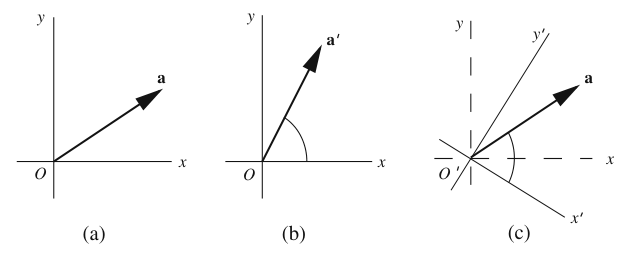
\includegraphics[scale = 1]{imgs/tps.png}
    \caption{(a) Sistema Original. (b) Transformación Activa. (c) Transformación Pasiva}
    \label{fig:transfor}
\end{figure}

\subsection[short]{Teorema de Noether}

La conexión entre la invariancia y la conservación en sistemas en los que no aparecen coordenadas ignorables esta dada mediante el \textit{Teorema de Noether}. Este teorema establece que si $L$ es invariante bajo una familia de transformaciones, su sistema dinámico posee una constante de movimiento, la cual puede ser encontrada en términos de $L$ y las transformaciones.
\vspace{2cm}
\\
Este teorema involucra familias de transformaciones continuas $\psi(\epsilon)$, dado que $L$ es una función que pertenecen a $\mathbf{T}\mathbb{Q}$ entonces es necesario estudiar las transformaciones en este espacio, esto también es debido a que transformaciones sobre $\mathbb{Q}$ implican transformaciones en $\mathbf{T}\mathbb{Q}$. Plantando una transformación pasiva, cada valor de $q$ (cada conjunto de coordenadas $q^{\alpha}$) cambia a otro $q(\epsilon)$ mediante cada valor de $\epsilon$, entonces cada trayectoria $q(t)$ cambia sus coordenadas por otras nuevas $q(t,\epsilon)$, esto permite expresar entonces a $\dot{q}(t,\epsilon)$ como  la derivada parcial de $q(t,\epsilon)$ respecto a $t$. Esto permite escribir la transformación del Lagrangiano

\begin{gather*}
    L(\xi,t) = L_\epsilon(\mathbf{T}\psi(\xi),t) 
\end{gather*}
Donde $\mathbf{T}\psi(\epsilon)$ describe una transformación en $\mathbf{T}\mathbb{Q}$ y $\xi = (q,\dot{q})$ es un punto en $\mathbf{T}\mathbb{Q}$. También es valido expresar 

\begin{gather*}
    L(q,\dot{q},t) = L\left(\psi(q),\frac{\partial \psi(q)}{\partial t},t\right)
\end{gather*}

Debido a que $L$ es covariante ante transformaciones entonces su derivada respecto a $\epsilon$ debe ser cero.

\begin{gather*}
    \frac{\partial L_\epsilon}{\partial \epsilon} = \frac{\partial L_\epsilon}{\partial q^{\alpha}}\frac{\partial q^{\alpha}}{\partial \epsilon} + \frac{\partial L_\epsilon}{\partial \dot{q}^{\alpha}}\frac{\partial \dot{q}^{\alpha}}{\partial \epsilon}  = 0
\end{gather*}
Recordando la propiedad de la Eq.\ref*{eq:prop}

\begin{gather*}
    \frac{\partial L_\epsilon}{\partial q^{\alpha}}\frac{\partial q^{\alpha}}{\partial \epsilon} + \frac{\partial L_\epsilon}{\partial \dot{q}^{\alpha}}\frac{d}{dt}\frac{\partial q^{\alpha}}{\partial \epsilon}  = 0
\end{gather*}
El segundo término de la parte izquierda se puede expresar en términos del producto de una derivada si se considera que 

\begin{gather*}
    \frac{d}{dt}\left(\frac{\partial L_\epsilon}{\partial \dot{q}^{\alpha}}\frac{\partial q^{\alpha}}{\partial \epsilon}\right) = \frac{\partial L_\epsilon}{\partial \dot{q}^{\alpha}}\frac{d}{dt}\frac{\partial q^{\alpha}}{\partial \epsilon} + \frac{\partial q^{\alpha}}{\partial \epsilon}\frac{d}{dt}\frac{\partial L_\epsilon}{\partial \dot{q}^{\alpha}}\\
    \frac{d}{dt}\left(\frac{\partial L_\epsilon}{\partial \dot{q}^{\alpha}}\frac{\partial q^{\alpha}}{\partial \epsilon}\right) - \frac{\partial q^{\alpha}}{\partial \epsilon}\frac{d}{dt}\frac{\partial L_\epsilon}{\partial \dot{q}^{\alpha}} = \frac{\partial L_\epsilon}{\partial \dot{q}^{\alpha}}\frac{d}{dt}\frac{\partial q^{\alpha}}{\partial \epsilon}
\end{gather*}
Remplazando 

\begin{gather*}
    \frac{\partial L_\epsilon}{\partial q^{\alpha}}\frac{\partial q^{\alpha}}{\partial \epsilon} + \frac{d}{dt}\left(\frac{\partial L_\epsilon}{\partial \dot{q}^{\alpha}}\frac{\partial q^{\alpha}}{\partial \epsilon}\right) - \frac{\partial q^{\alpha}}{\partial \epsilon}\frac{d}{dt}\frac{\partial L_\epsilon}{\partial \dot{q}^{\alpha}} = 0
\end{gather*}
Agrupando y remplazando la transformación $q^{\alpha} = \psi(q^{\alpha})$

\begin{gather*}
    \left(\frac{\partial L_\epsilon}{\partial q^{\alpha}} - \frac{d}{dt}\frac{\partial L_\epsilon}{\partial \dot{q}^{\alpha}} \right) \frac{\partial \psi(q^{\alpha})}{\partial \epsilon} + \frac{d}{dt}\left(\frac{\partial L_\epsilon}{\partial \dot{q}^{\alpha}}\frac{\partial \psi(q^{\alpha})}{\partial \epsilon}\right)   = 0
\end{gather*}
El primer término de esta ecuación ya es cero, debido a que son las ecuaciones de Euler-Lagrange, por lo tanto la expresión para la derivada queda expresada como

\begin{gather*}
    \frac{\partial L_\epsilon}{\partial \epsilon} = \frac{d}{dt}\left(\frac{\partial L_\epsilon}{\partial \dot{q}^{\alpha}}\frac{\partial \psi(q^{\alpha})}{\partial \epsilon}\right) 
\end{gather*}
Evaluando la derivada en $\epsilon = 0$ se obtiene su variacional, por otro lado el funcional $\psi$ siempre estará restringido por la familia de transformaciones que inicia con la transformación identidad $\psi(\epsilon = 0) = q$.

\begin{gather}
    \label{eq:vartl}\delta L_\epsilon = \frac{d}{dt}\left(\frac{\partial L_\epsilon}{\partial \dot{q}^{\alpha}}\delta q^{\alpha}\right)  = 0
\end{gather}
Esto nos indica que el argumento de la derivada será una constante de movimiento  

\begin{gather}
    \label{eq:noet}\Gamma = \frac{\partial L_\epsilon}{\partial \dot{q}^{\alpha}}\delta q^{\alpha}
\end{gather}
\\
Esto demuestra el teorema de Noether, el cual indica que si $L$ es invariante ante transformaciones puntuales (transformaciones sobre $\mathbb{Q}$), entonces existirá una constante de movimiento dada por $\Gamma$. Esto implica que a cada simetría de $L$ corresponde una constante del movimiento.\newline
Para el caso en que $L$ no se un invariante entonces la diferencia entre dos Lagrangianos es la derivada total de una función respecto al tiempo, tal como se demostró en la Eq.\ref*{eq:difl}.

\begin{gather*}
    L_\epsilon = L + \frac{d\Phi}{dt}
\end{gather*}
Donde $\Phi$ es una función de $q$, $t$ y $\epsilon$, entonces el variacional de $L$ será 

\begin{gather*}
    \delta L_\epsilon = \frac{d}{dt}\delta \Phi
\end{gather*}
Remplazando el valor de $\delta L_\epsilon$ (Eq. \ref*{eq:vartl}) se obtiene

\begin{gather*}
    \frac{d}{dt}\left(\frac{\partial L_\epsilon}{\partial \dot{q}^{\alpha}}\delta q^{\alpha}\right) = \frac{d}{dt}\delta \Phi
\end{gather*}
Por tanto, la constante de movimiento es 

\begin{gather}
    \Gamma = \frac{\partial L_\epsilon}{\partial \dot{q}^{\alpha}}\delta q^{\alpha} - \delta \Phi
\end{gather}

\subsection[short]{Ejemplo}

\end{document}
